\section{Experimental Results} \label{sec:experiments}

The goal of this section is to evaluate the proposed control framework and the adaptation to the original SC method. iTo this end, we define the following metrics:
\begin{itemize}
    \item \textit{average stage cost}: this performance metric is computed by averaging the stage cost evaluated at each time step. Task duration and cost scheduling is kept fixed among all the experiments.  
    \item \textit{cumulative constraints violation}: as each barrier function is, by definition, negative outside of the safe set, we define the following metric as a proxy for the size of the constraint violation along the duration of an experiment:
    \begin{equation*}
        \Delta^{i}_{tot} = \sum\limits_{t=0}^{T_{exp}} \max(0, -h^i(\vect{x}_t)),
    \end{equation*}
    referring to the $i$th ZBF.
    \item \textit{average interaction wrench}: average wrench which is exerted on the environment during the execution of the task
    \item \textit{dissipated power}: during an ideal interaction with an articulated object, power is minimally dissipated. Therefore, we use the dissipated power as an efficiency metric:
    \begin{equation}
        P_{diss} = \sum\limits_{0}^{T_{exp}} -\command^T \boldsymbol{\tau}_{ext}.
    \end{equation}
\end{itemize}
The simulation experiments are conducted on a dynamic manipulator model as described by \eqn \eqref{eq:eom}. To this end, we use the Raisim physics engine \cite{raisim}. The manipulation tasks consist of maneuvering different articulated objects. The articulated objects in the task are a \textit{shelf}, \textit{dishwasher}, \textit{microwave} and \textit{drawer} as shown in \fig\ref{fig:object_manipulation}. They differ in type and orientation of the joint. The \textit{shelf} and \textit{microwave} have a vertical revolute joint, the \textit{dishwasher} has a horizontal revolute joint, while the \textit{drawer} has a horizontal prismatic joint. The simulated manipulator is controlled using a PI low-level velocity controller running at 1KHz. Imperfect velocity control is modeled by compensating only 90\% of the gravity terms.
  
\begin{figure}[t]
\centering
  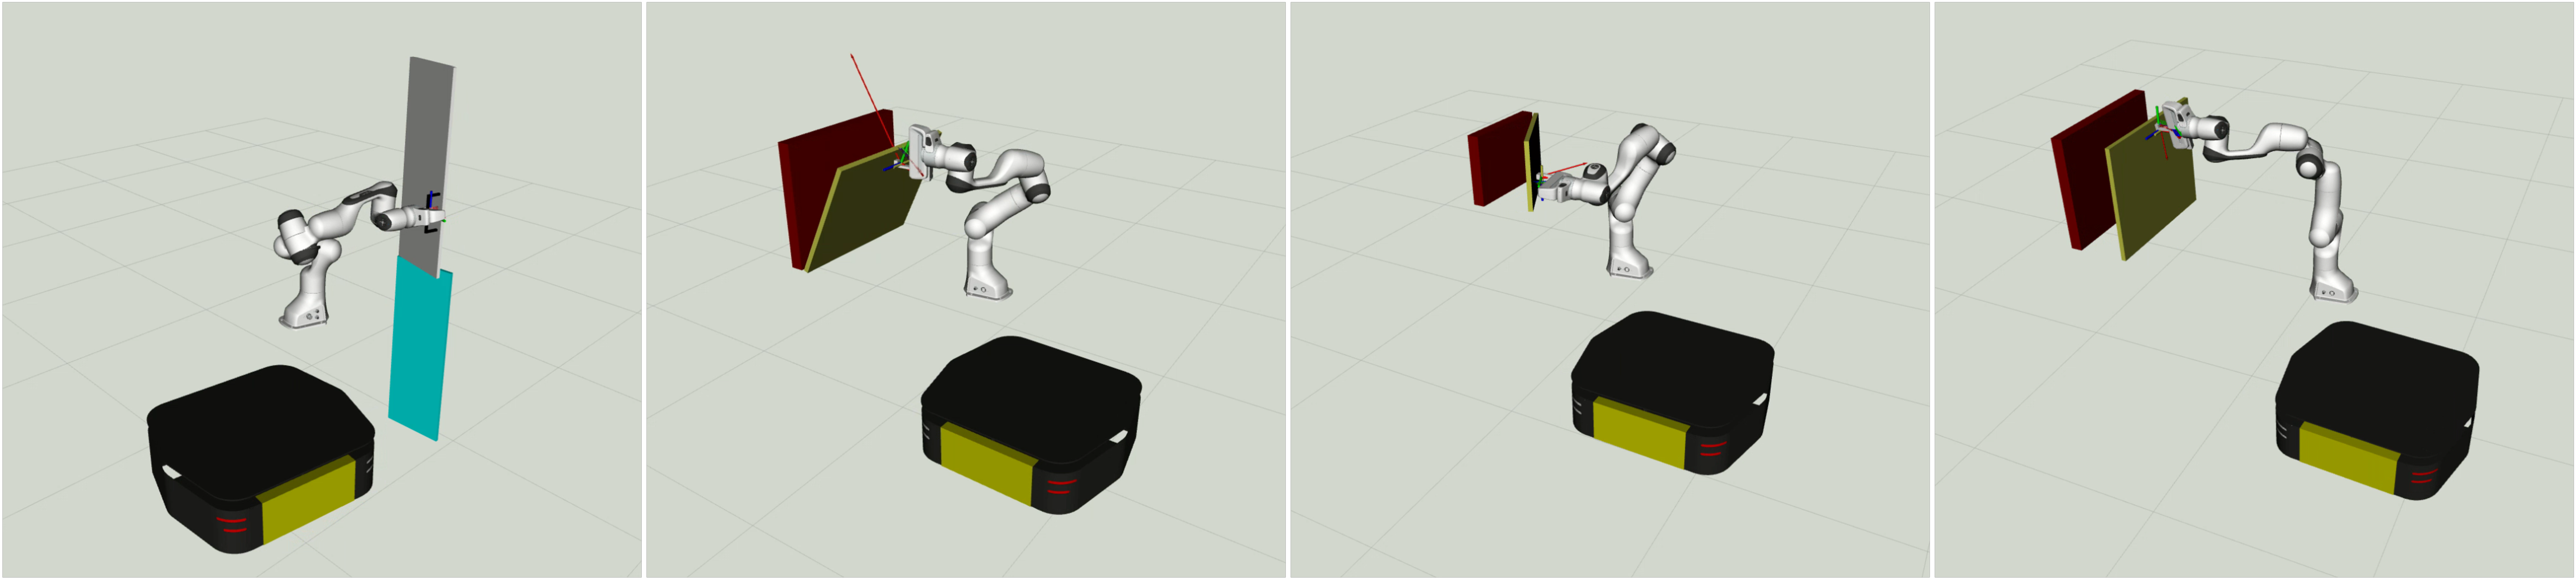
\includegraphics[width=\columnwidth]{framework_manipulation/figures/mosaics/articulated_objects_sim.pdf}
  \caption{The four articulated objects used in our simulation evaluations. From left to right: shelf, dishwasher, microwave, drawer.} \label{fig:object_manipulation}
\end{figure}

\subsection{Power consumption}
In this experiment we look at the effect of the power term in the task execution. As we can see in \fig \ref{fig:power_cost_comparison}, the power cost is effective in decreasing the energy dissipation during the manipulation task. For each of the experiments where the power cost is active we set $w_p=10$ and $p_{max} = 0.0$. For all experiments we use $50$ samples as they are a good trade-off between control-frequency and performance. We observe that in all experiments the robot is able to accomplish the task (fully open the articulated object). 

\begin{figure}[t]
\centering
  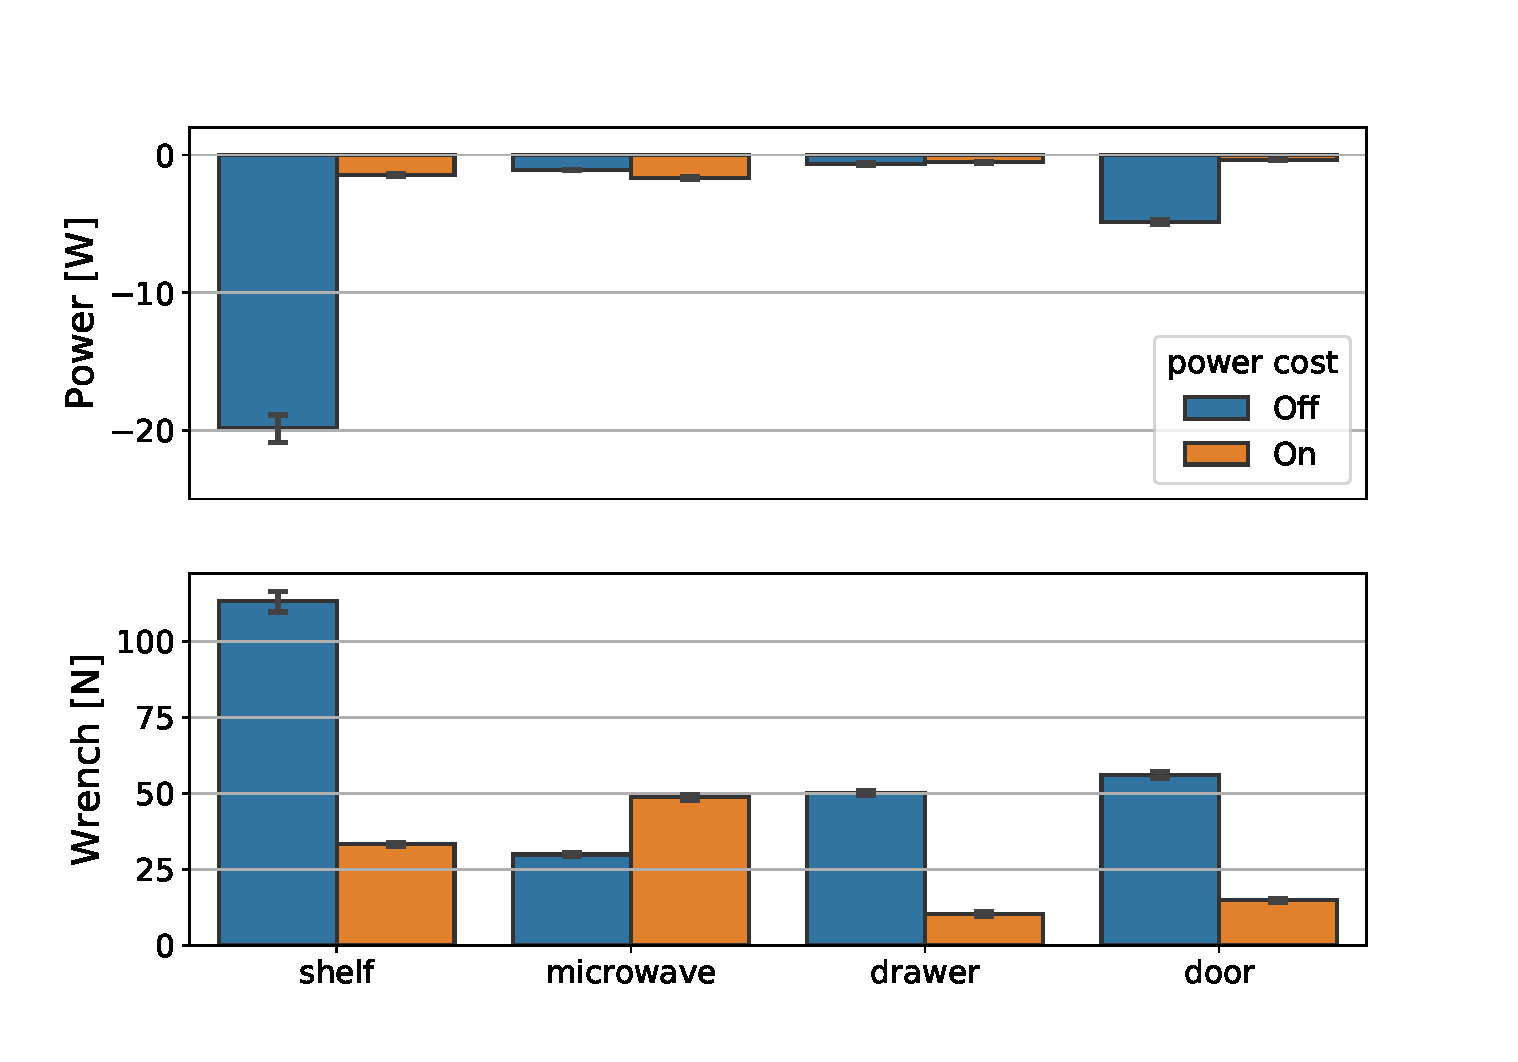
\includegraphics[width=\columnwidth]{figures/methods_comparison/power_cost.pdf}
  \caption{Power dissipated and wrench norm for each of the manipulated objects.} \label{fig:power_cost_comparison}
\end{figure}


\subsection{Comparison of methods}
We evaluate the control framework for a challenging interaction scenario. In all experiments, the robot starts in a configuration that is close to the arm's joint limits and self-collision. The base of the robot is at $(-3.0, -3.0)$, outside of the prescribed position limits of $[(2.0, 2.0), (-2.0, -2.0)]$. We perform 10 experiments for each articulated object and we compare four control adaptations:
\begin{itemize}
    \item \textit{no\textunderscore filter}: only sampling is used to generate velocity commands,
    \item \textit{filter\textunderscore out}: before sending the velocity command to the low-level controller, it is filtered using the high rate FILTER-QP,
    \item \textit{filter\textunderscore in}: the Sequential FILTER-QP is used in the low-rate block. The full input sequence is passed through the FILTER-QP before being sent to the low-level controller as described in \algo \ref{algo:sequential_qp}.
    \item \textit{filter\textunderscore in\textunderscore out}: the full cascaded architecture (see \fig \ref{fig:cascaded_architecture}) is deployed, combining the previous two methods.
\end{itemize}
The results of the experiments are summarized in \fig \ref{fig:methods_comparison}. In all cases, filtering the velocity commands has a beneficial effect. The drastic reduction of cumulative joint limit violations shows that closing the loop between the filter and the sampling allows the controller to quickly generate trajectories that recover from constraint violations. We can also observe a reduction in self-collision and reach constraint violations, but in this case the improvement of  \textit{filter\textunderscore in\textunderscore out} with respect to \textit{filter\textunderscore in} is not as prominent. We think that this is due to a low chance of getting into self-collision given the task and robot shape. The robustness provided by the energy tank is particularly useful when something unexpected happens. In the following we design a challenging scenario which, without the tank, could lead to dangerous behaviors. 
\begin{figure}[t]
\centering
\hspace*{-0.2cm} 
\begin{subfigure}{1\columnwidth}
    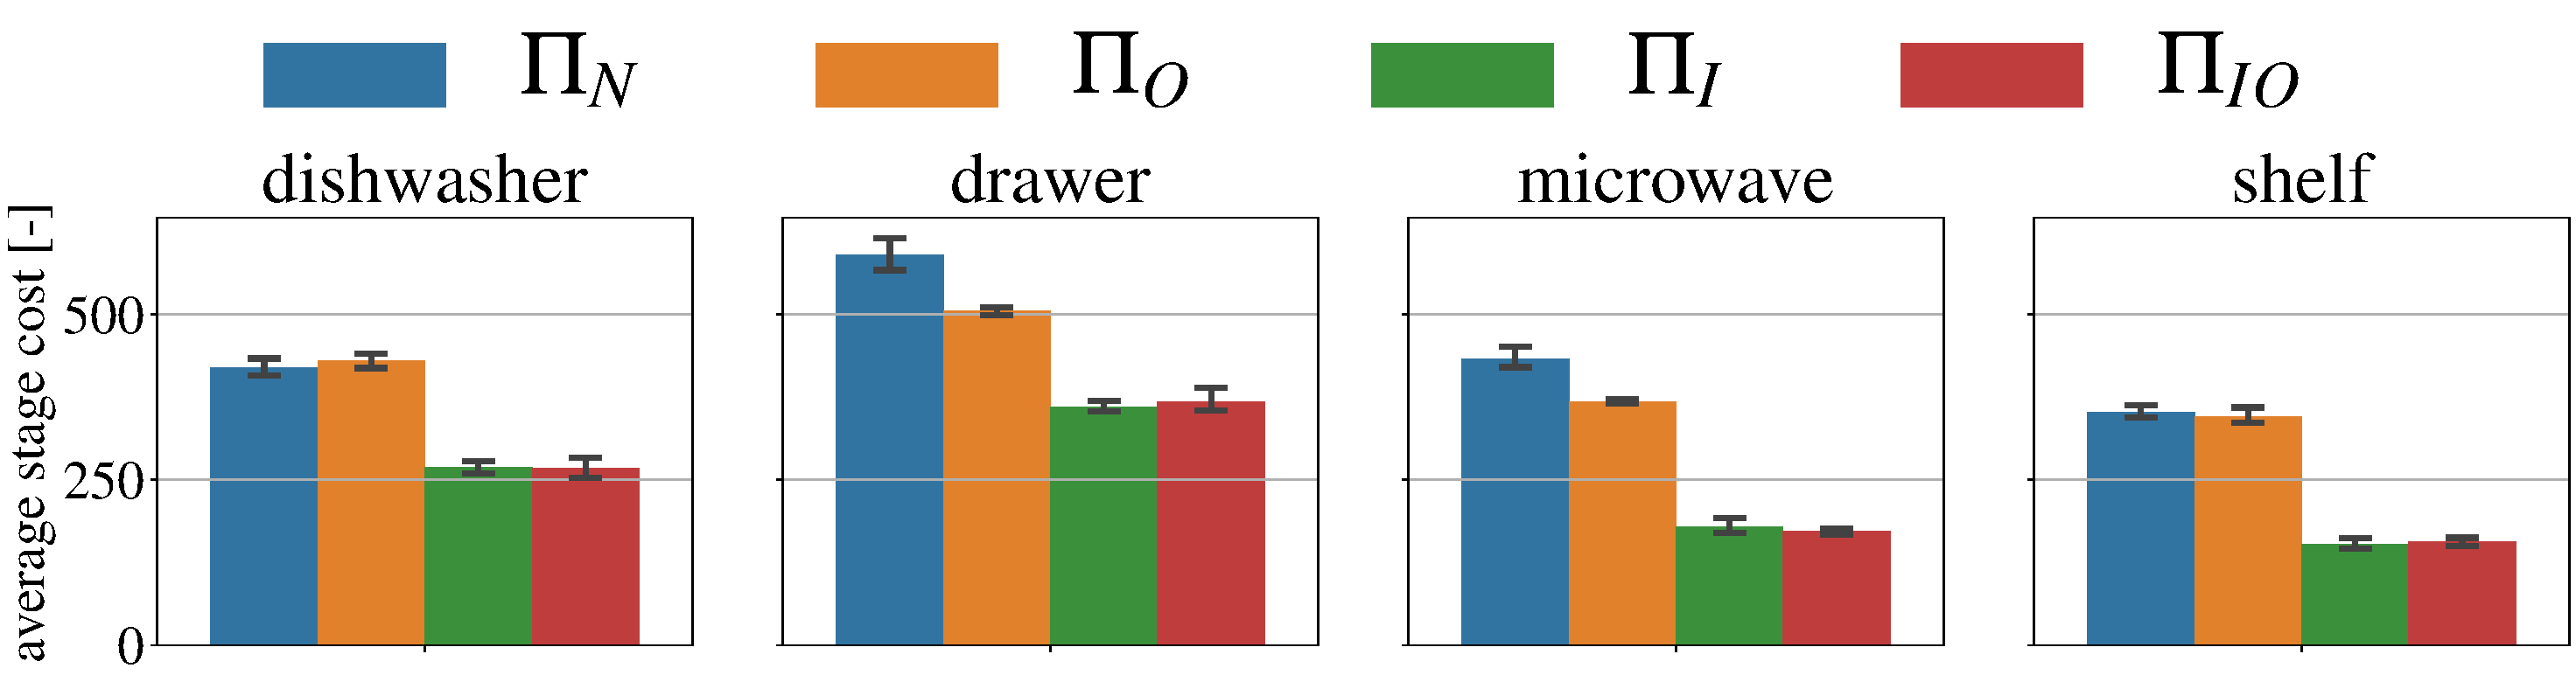
\includegraphics[width=\linewidth]{figures/methods_comparison/average_stage_cost.pdf}
\end{subfigure}%
\hfill
\hspace*{-0.2cm} 
\begin{subfigure}{1\columnwidth}
    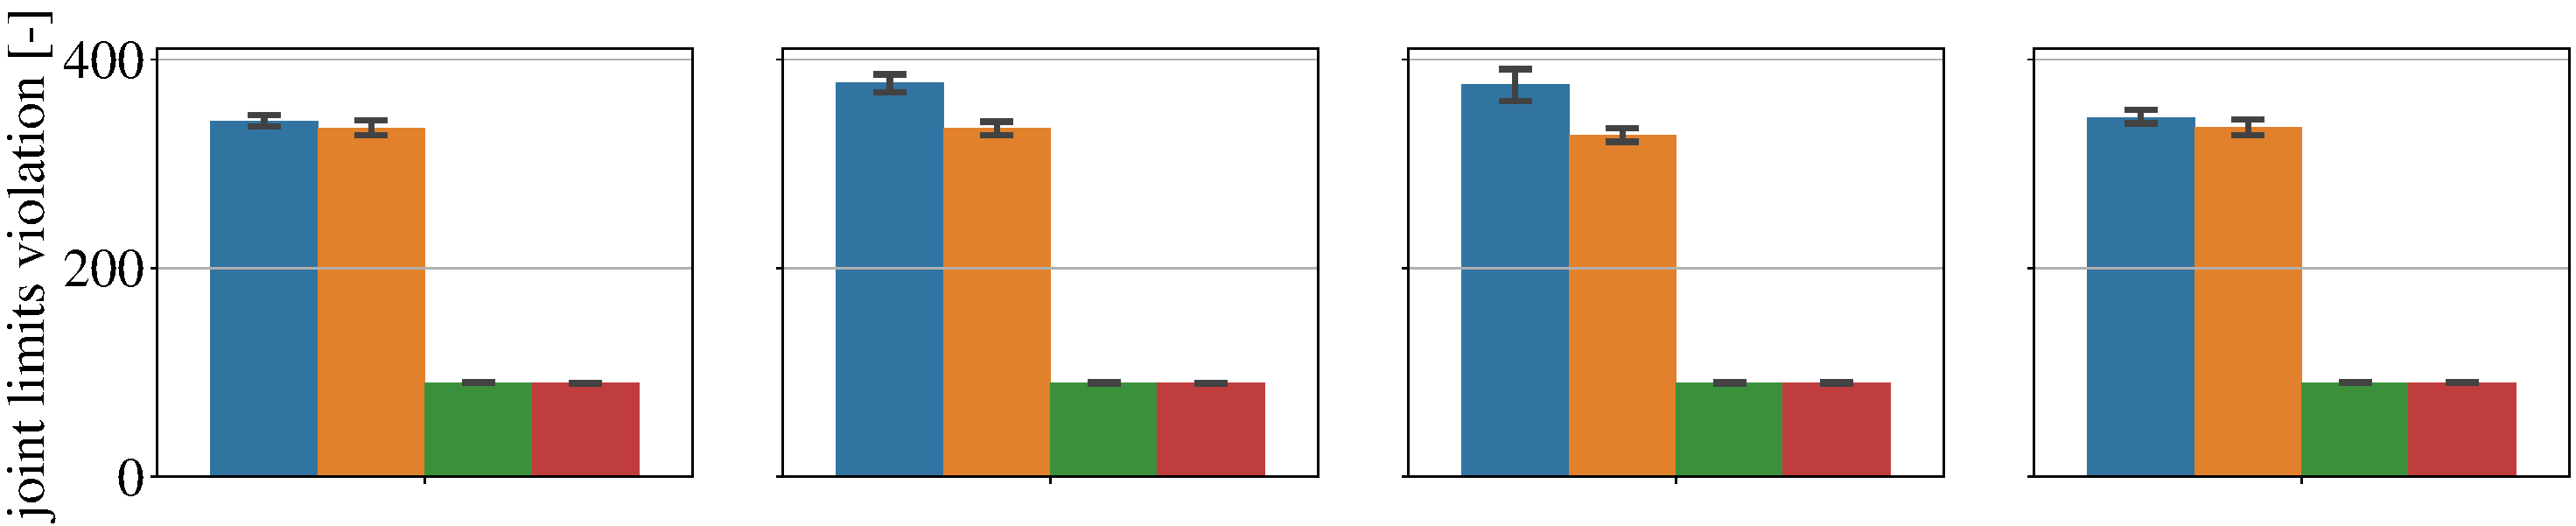
\includegraphics[width=\linewidth]{figures/methods_comparison/joint_limits.pdf}
\end{subfigure}%
\hfill
\hspace*{-0.2cm} 
\begin{subfigure}{1\columnwidth}
    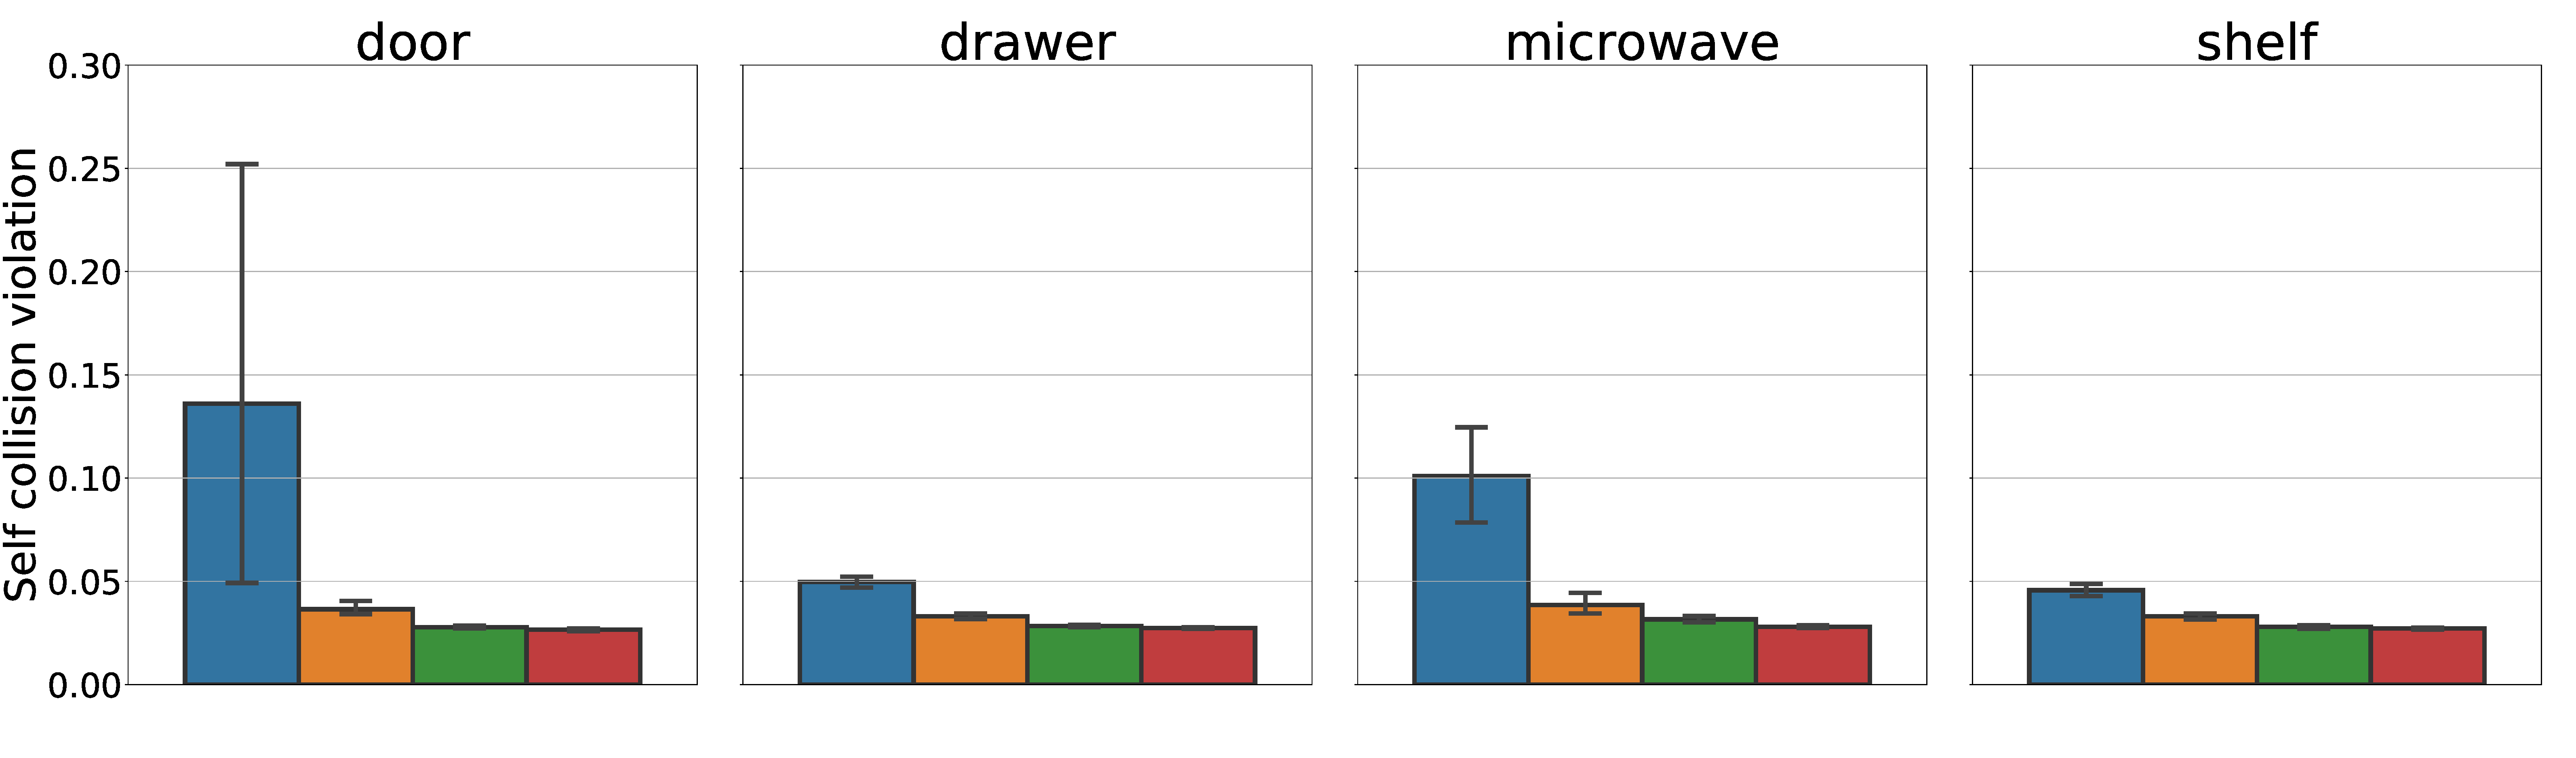
\includegraphics[width=\linewidth]{figures/methods_comparison/self_collision.pdf}
\end{subfigure}
\hspace*{-0.2cm} 
\begin{subfigure}{1\columnwidth}
    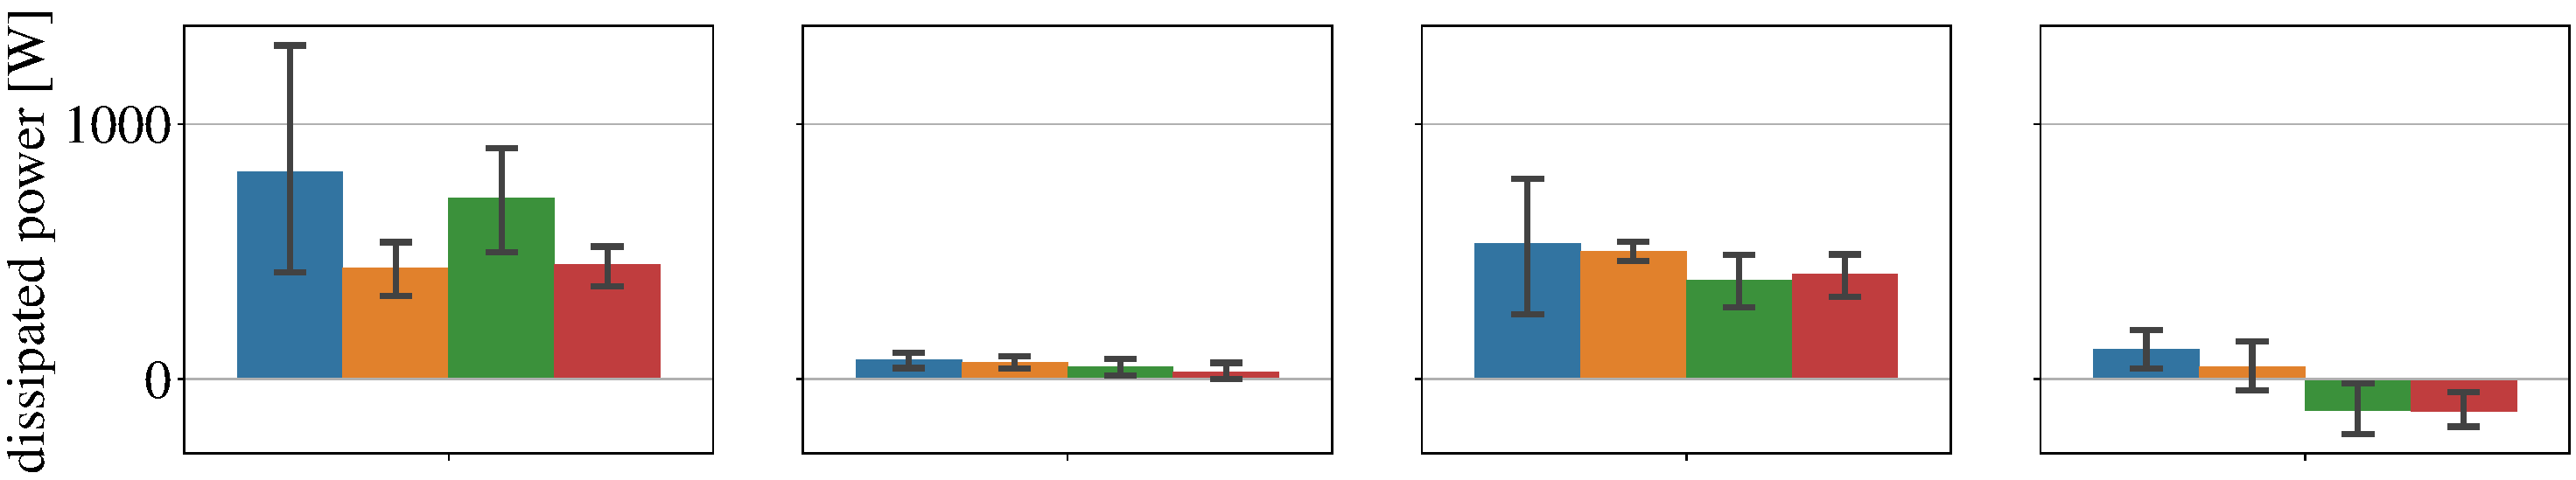
\includegraphics[width=\linewidth]{figures/methods_comparison/dissipated_power.pdf}
\end{subfigure}
\hfill
\caption{Comparison between the different control methods when the FILTER-QP is used in different stages of the cascaded architecture. Results are separate by manipulation task. The self-collision metric accounts also for the arm-reach constraint as they share the same implementation.}\label{fig:methods_comparison}
\end{figure}

\subsection{Robust interaction}
We aim to show that the tank is effective in limiting the dissipated power and thus generating a stable and robust interaction behavior. In this experiment, the articulated object becomes stuck while the robot is interacting with it. We fix the object position for $5s$. After this time the object is released and is free to move within its limits. From the results in \fig\ref{fig:tank_comparison}, we can note that when the FILTER-QP is turned off and therefore no passivity is ensured, the negative power flow is not bounded, leading to high interaction wrenches. On the other hand, when the energy tank is used, only a maximal amount of energy, namely that stored in the tank, can be used, regulating the overall interaction wrench.    

%\begin{figure}[t]
%\centering
%\hspace*{-0.0cm} 
%\begin{subfigure}{1.0\columnwidth}
%    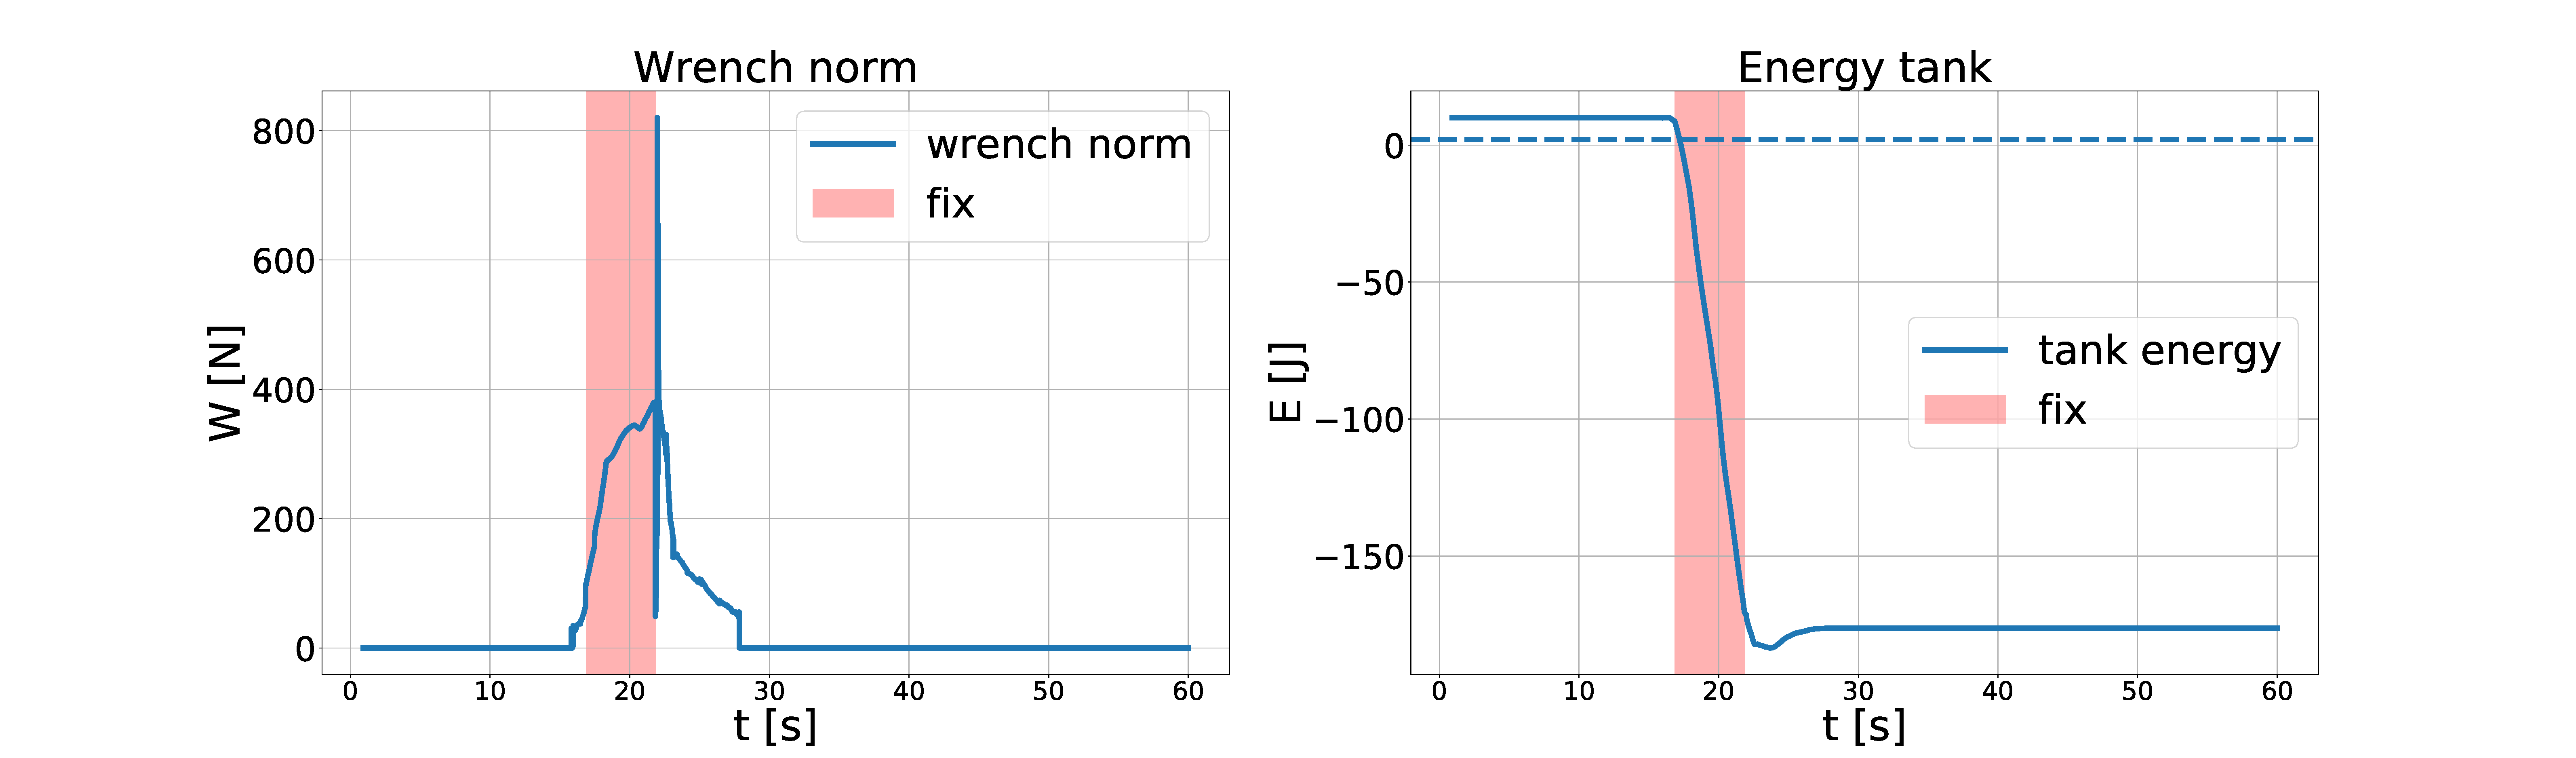
\includegraphics[trim=250 0 250 0, clip,width=\linewidth]{figures/fix_experiment/wrench_tank_without_tank.pdf}
%    \caption{without tank}
%\end{subfigure}
%\hspace*{-0.0cm} 
%\begin{subfigure}{1.0\columnwidth}
%    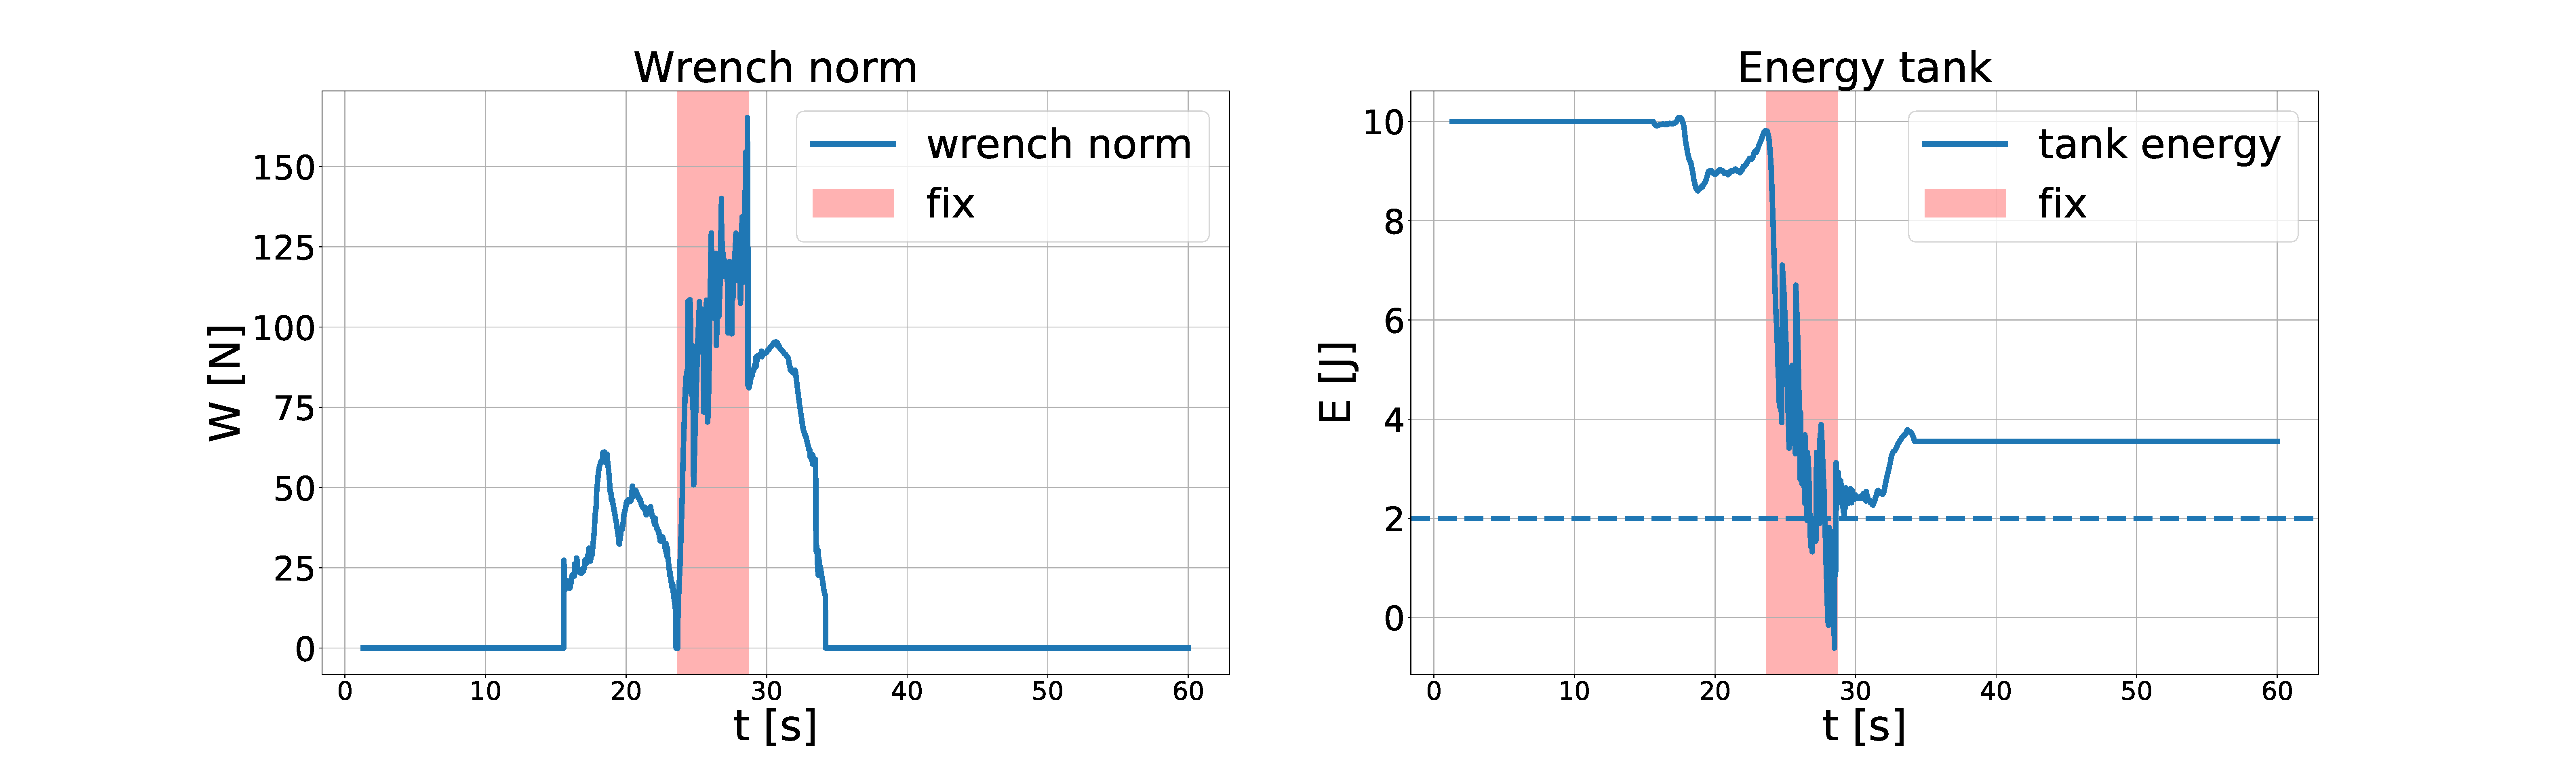
\includegraphics[trim=250 0 250 0, clip,width=\linewidth]{figures/fix_experiment/wrench_tank_with_tank.pdf}
%    \caption{with tank}
%\end{subfigure}
%\hfill
%\caption{The figure shows the interaction wrench and energy in the tank during the task execution. The shaded area is the interval of time during which the articulated object is fixed.  }\label{fig:tank_comparison}
%\end{figure}

\begin{figure}[t]
\centering
\hspace*{-0.0cm} 
\begin{subfigure}{1.0\columnwidth}
    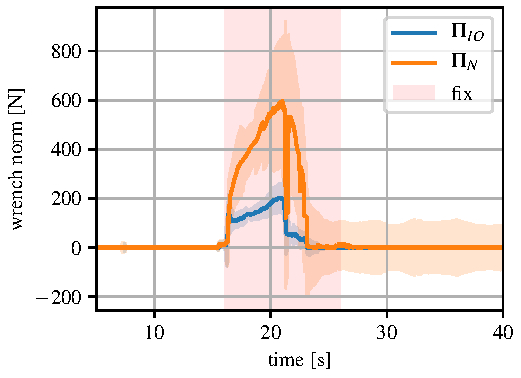
\includegraphics[width=\linewidth]{figures/fix_experiment/wrench_with_without_tank.pdf}
\end{subfigure}
\hspace*{-0.0cm} 
\begin{subfigure}{1.0\columnwidth}
    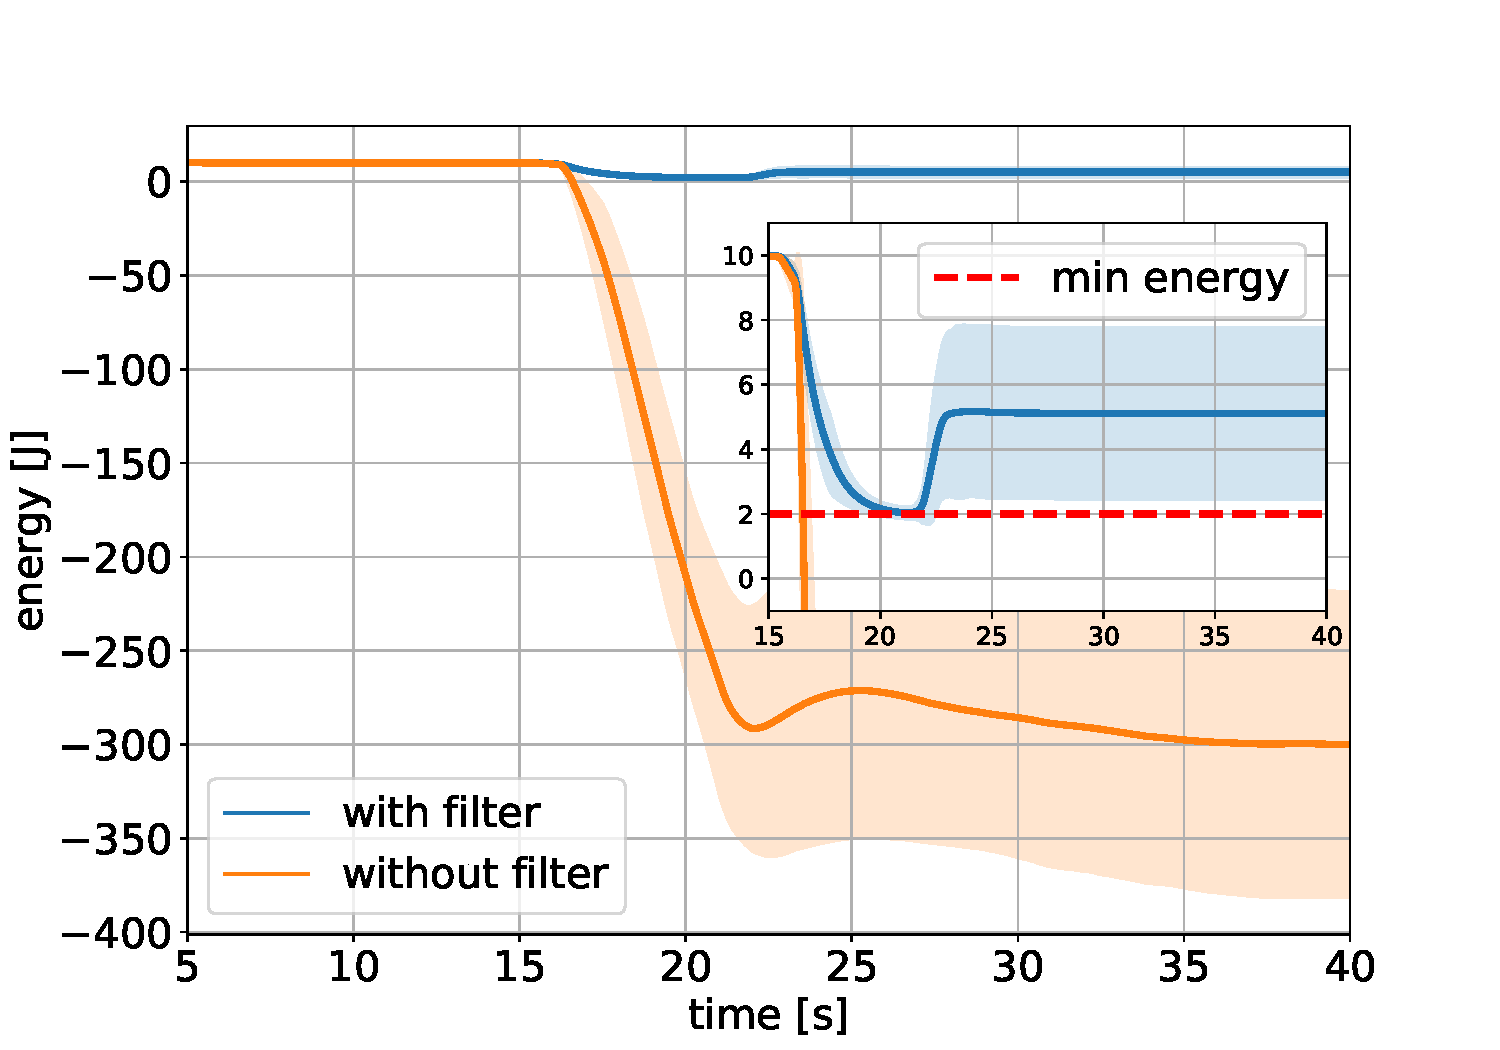
\includegraphics[width=\linewidth]{figures/fix_experiment/energy_with_without_tank.pdf}
\end{subfigure}
\hfill
\caption{The figure shows the interaction wrench and energy in the tank during the task execution. The shaded area is the interval of time during which the articulated object is fixed.  }\label{fig:tank_comparison}
\end{figure}

\subsection{Real world experiments}
Our RoyalPanda test platform consists of a holonomic mobile base equipped with a 7-DOF manipulator. The robot's wrist mounts a custom set of fingers as shown in \fig\ref{fig:custom_fingers}. This hardware adaptation simplifies the problem without limiting the capabilities of the platform. We run the presented algorithm on a Intel Core i7-8550U quad-core processor (1.8 GHz, up to 4.0 GHz) and use 8 threads for parallel forward sampling of rollouts. All control parameters are summarized in \tab \add{add table of parameters}. The target velocity commands are tracked by a PI controller which converts these into motor torques. The omnidirectional base is controlled by sending velocity commands to the mecanum wheel controller. The arm's low-level controller runs at 1KHz while the base mecanum controller runs at 50Hz. The FILTER-QP is solved efficiently using the \texttt{osqp} C++ library \cite{osqp}. We measure an average solving time of $\approx 0.1$ ms.  


The goal of the experiment is to demonstrate that the algorithm can be deployed on a real platform at high control rates. For this purpose, we perform a door opening experiment. The door and the robot base are tracked via a VICON system, eliminating the need for precise state estimation. We plan to remove this limitation in future work. In order to qualitatively evaluate the algorithm's replanning capabilities, we disturb the manipulator during the opening phase, releasing the contact between the handle and the finger. As we can see in the accompanying video, the controller is able to re-plan a feasible trajectory to the handle and successfully perform the task.